\section{Results and Findings by Task}

This section presents the results obtained for each of the six defined tasks. For supervised
tasks, model performance is compared before and after preprocessing in order to evaluate the
impact of scaling and feature preparation. For exploratory tasks, the findings are presented
through clustering quality, association rules, and interpretable feature-based insights.

\subsection{Task 1: Predicting Whether a News Article Will Be Popular}

Task 1 was formulated as a binary classification problem, where an article was labeled as
\textit{popular} if its number of shares was greater than or equal to the median value
(1400), and \textit{unpopular} otherwise. Eight classification models were evaluated before and
after preprocessing.

\subsubsection*{Results Before Preprocessing}

\begin{table}[H]
\centering
\caption{Task 1 classification results before preprocessing}
\begin{tabular}{lccccc}
\toprule
Model & Accuracy & Precision & Recall & F1 & ROC-AUC \\
\midrule
Logistic Regression & 0.5970 & 0.6113 & 0.6724 & 0.6404 & 0.6318 \\
KNN & 0.5591 & 0.5870 & 0.5861 & 0.5866 & 0.5785 \\
SVM & 0.5055 & 0.5235 & 0.8152 & 0.6376 & 0.4507 \\
Decision Tree & 0.5654 & 0.5941 & 0.5859 & 0.5900 & 0.5639 \\
Random Forest & 0.6412 & 0.6531 & 0.6987 & 0.6751 & 0.6919 \\
Gradient Boosting & 0.6483 & 0.6566 & 0.7145 & 0.6843 & 0.7015 \\
AdaBoost & 0.6379 & 0.6483 & 0.7024 & 0.6743 & 0.6916 \\
Naive Bayes & 0.5176 & 0.6750 & 0.1851 & 0.2905 & 0.6208 \\
\bottomrule
\end{tabular}
\end{table}

\subsubsection*{Results After Preprocessing}

\begin{table}[H]
\centering
\caption{Task 1 classification results after preprocessing}
\begin{tabular}{lccccc}
\toprule
Model & Accuracy & Precision & Recall & F1 & ROC-AUC \\
\midrule
Logistic Regression & 0.6305 & 0.6412 & 0.6982 & 0.6685 & 0.6762 \\
KNN & 0.5871 & 0.6181 & 0.5918 & 0.6047 & 0.6111 \\
SVM & 0.5457 & 0.5862 & 0.5053 & 0.5428 & 0.5584 \\
Decision Tree & 0.5639 & 0.5921 & 0.5871 & 0.5896 & 0.5622 \\
Random Forest & 0.6409 & 0.6526 & 0.6996 & 0.6753 & 0.6926 \\
Gradient Boosting & 0.6469 & 0.6554 & 0.7133 & 0.6831 & 0.7016 \\
AdaBoost & 0.6379 & 0.6483 & 0.7024 & 0.6743 & 0.6916 \\
Naive Bayes & 0.5013 & 0.6716 & 0.1281 & 0.2152 & 0.6354 \\
\bottomrule
\end{tabular}
\end{table}

The best model before preprocessing was Gradient Boosting with an accuracy of 0.6483, and the
best model after preprocessing was again Gradient Boosting with an accuracy of 0.6469. Grouping models by family reveals a clear hierarchy:
\begin{itemize}[leftmargin=1.5em]
    \item \textbf{Tree-based ensembles} (RF, GB, AdaBoost): strongest group, accuracy 0.64--0.65
    \item \textbf{Linear models} (Logistic Regression): moderate, improved by scaling (0.60 $\to$ 0.63)
    \item \textbf{Distance-based} (KNN, SVM): weakest, most sensitive to feature scaling
    \item \textbf{Probabilistic} (Naive Bayes): poor recall due to violated independence assumptions
\end{itemize}
Preprocessing improved scale-sensitive models (Logistic Regression: +3.4\%, KNN: +2.8\%) but had negligible effect on tree-based ensembles, which are inherently scale-invariant.

\begin{figure}[H]
    \centering
    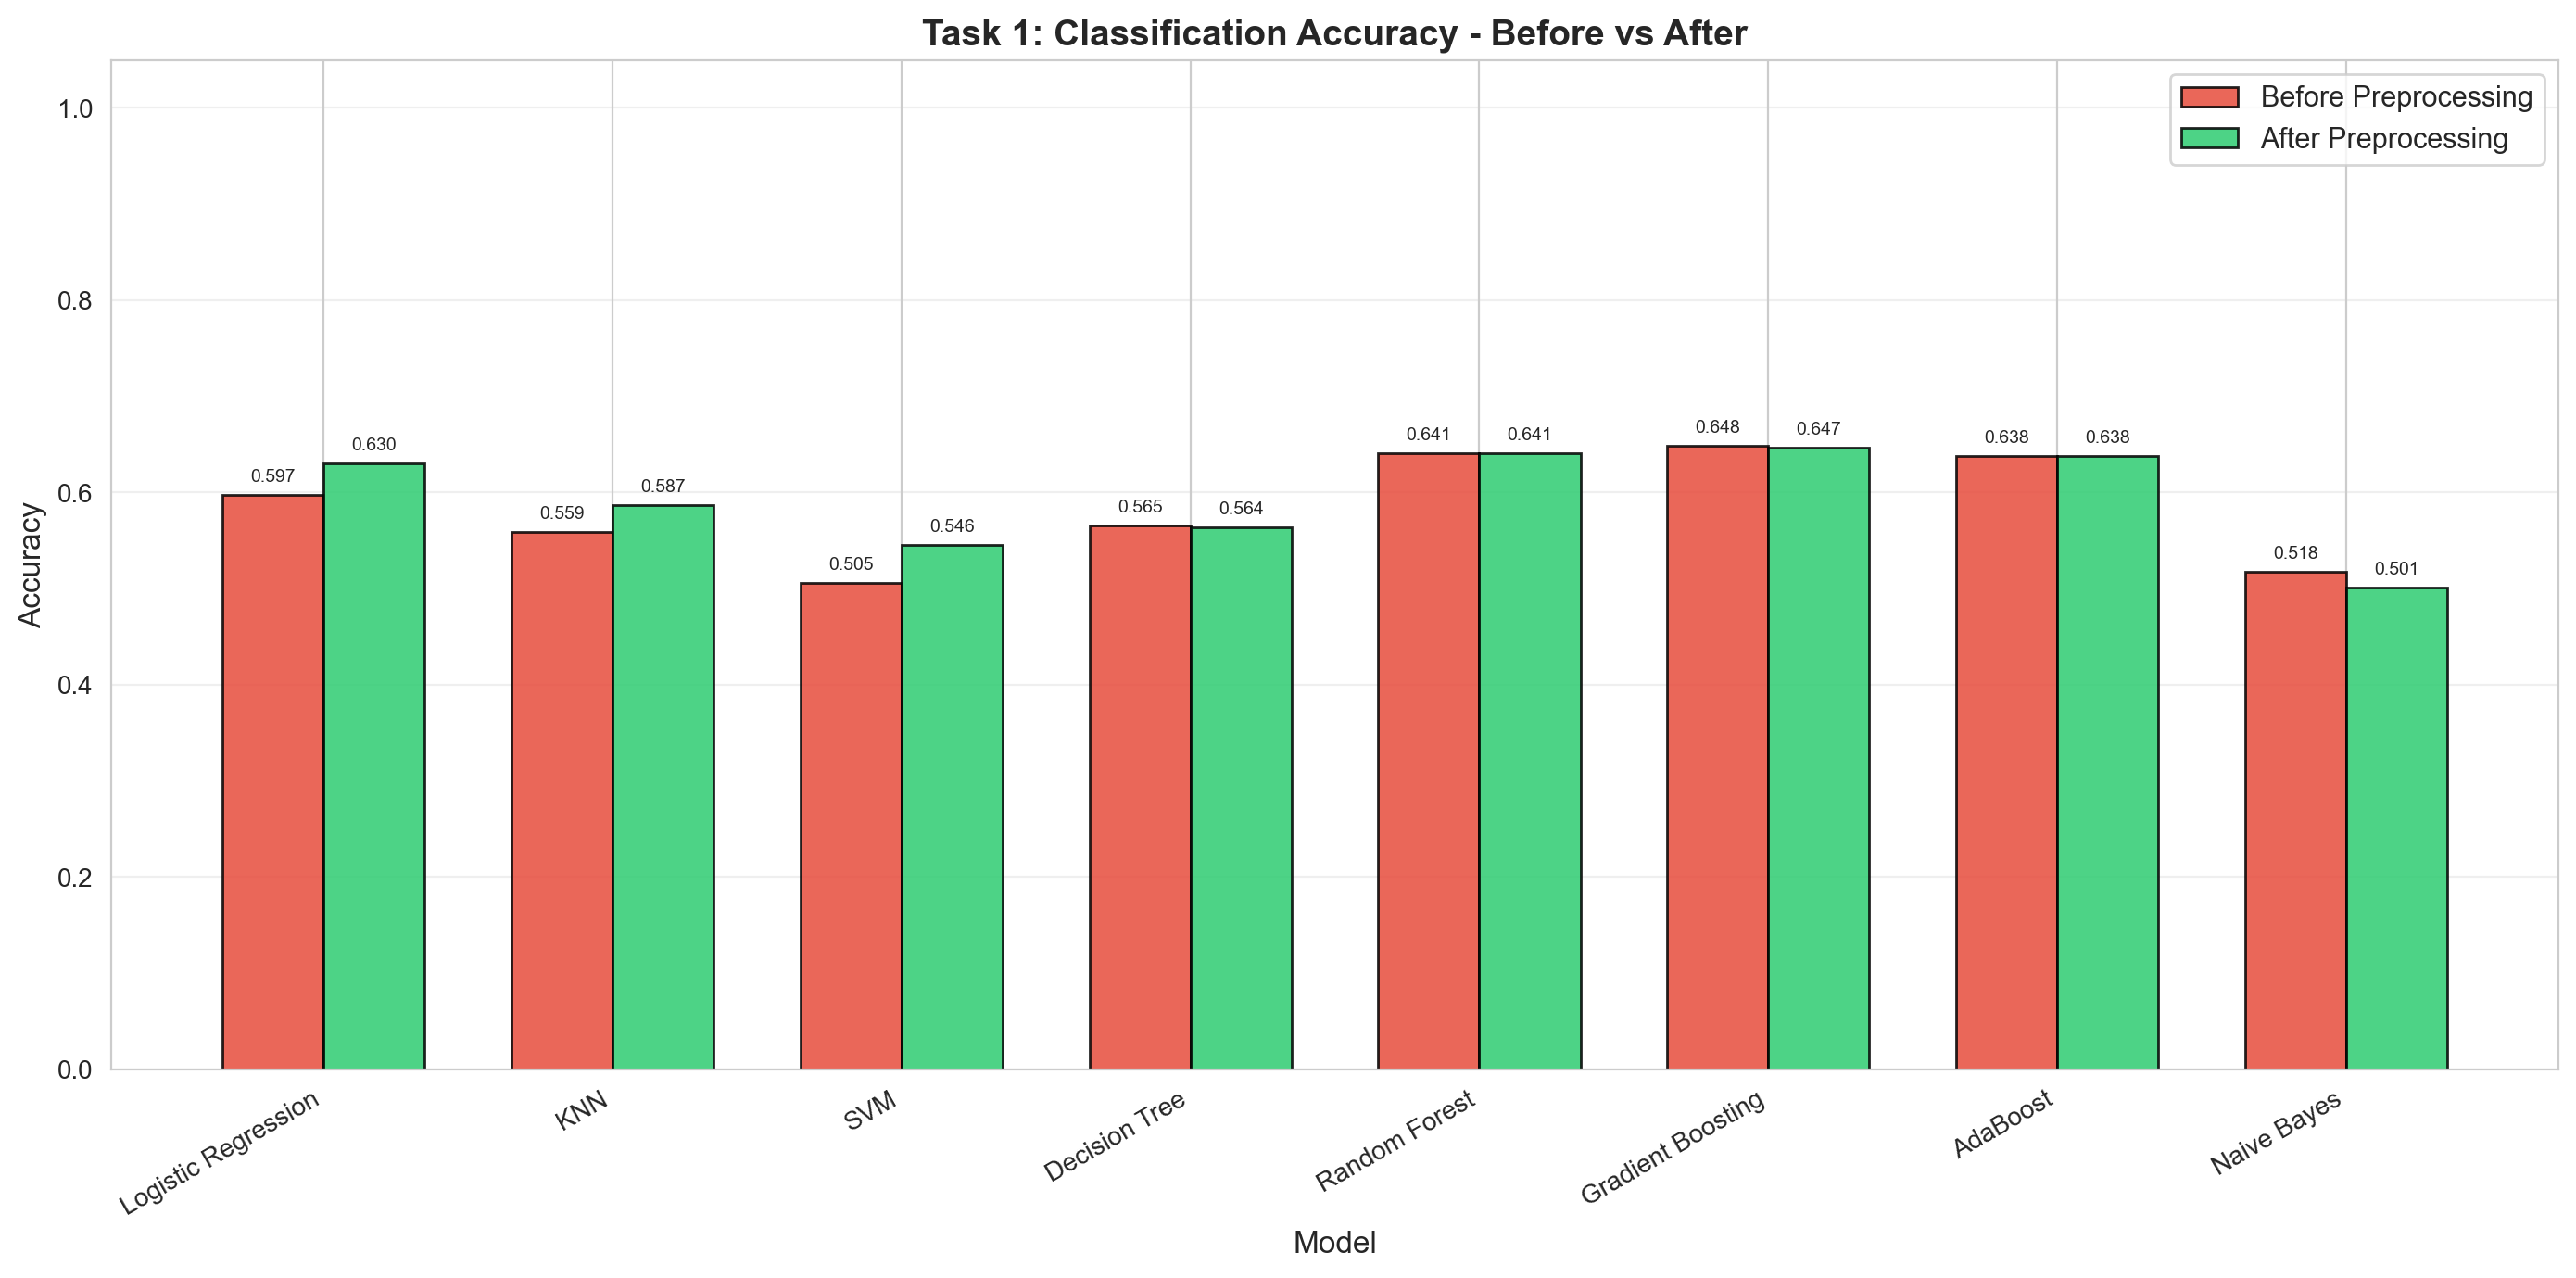
\includegraphics[width=0.7\textwidth]{figures/fig_task1_accuracy_comparison.png}
    \caption{Accuracy comparison for Task 1 classification models.}
\end{figure}

\begin{figure}[H]
    \centering
    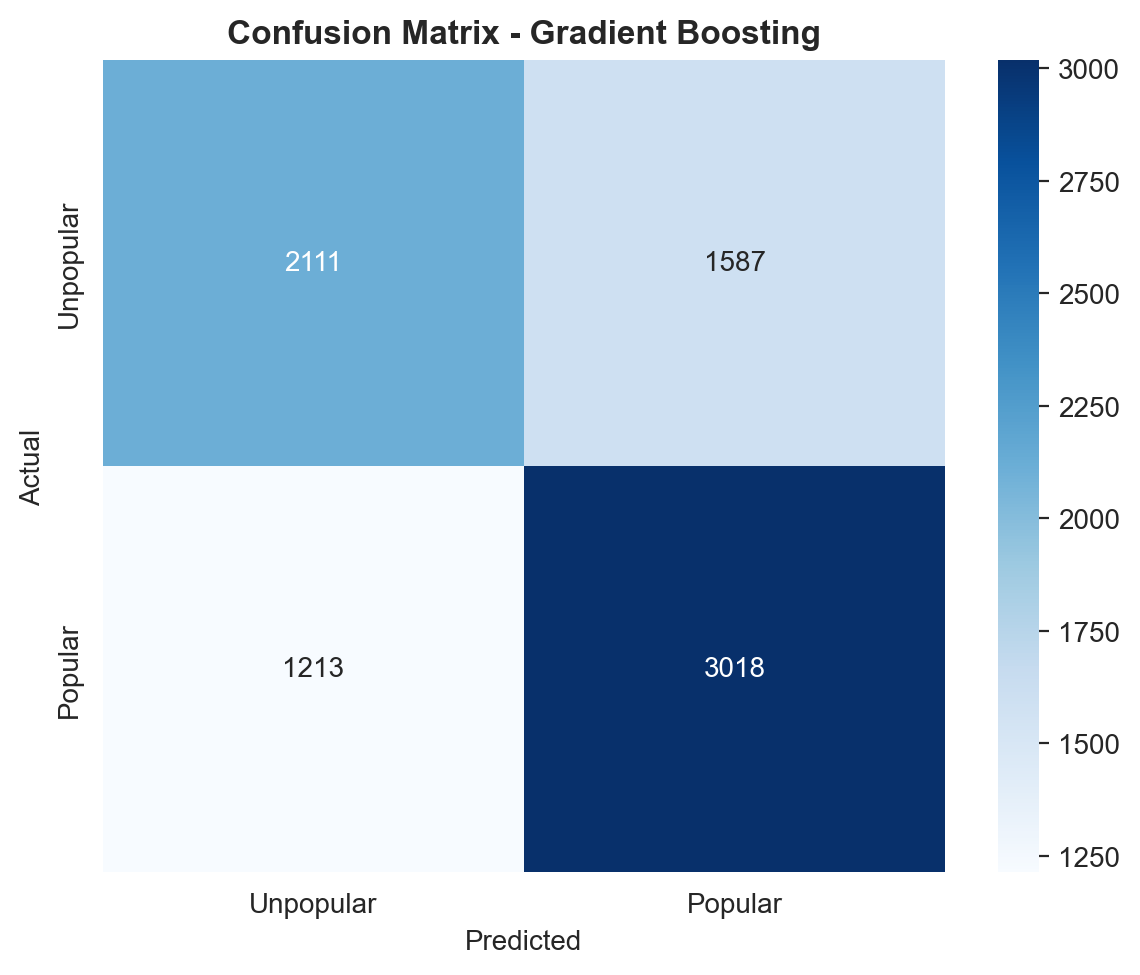
\includegraphics[width=0.65\textwidth]{figures/fig_task1_cm_best.png}
    \caption{Confusion matrix for the best Task 1 model.}
\end{figure}

\FloatBarrier

\subsection{Task 2: Predicting the Number of Shares an Article Will Receive}

Task 2 was formulated as a regression problem using the transformed target variable
$\log(1+\text{shares})$. Seven regression models were evaluated before and after preprocessing.

\subsubsection*{Results Before Preprocessing}

\begin{table}[H]
\centering
\caption{Task 2 regression results before preprocessing}
\begin{tabular}{lcccc}
\toprule
Model & RMSE$_{\log}$ & MAE$_{\log}$ & $R^2$ & RMSE$_{\text{orig}}$ \\
\midrule
Linear Regression & 0.8856 & 0.6574 & 0.1015 & 14646.95 \\
Ridge Regression & 0.8855 & 0.6573 & 0.1018 & 14646.83 \\
Lasso Regression & 0.8899 & 0.6636 & 0.0928 & 14652.19 \\
Decision Tree Regressor & 1.2644 & 0.9382 & -0.8314 & 18959.64 \\
Random Forest Regressor & 0.8727 & 0.6493 & 0.1275 & 14613.66 \\
Gradient Boosting Regressor & 0.8680 & 0.6408 & 0.1369 & 14631.04 \\
SVR & 2.6864 & 2.5036 & -7.2670 & 14994.45 \\
\bottomrule
\end{tabular}
\end{table}

\subsubsection*{Results After Preprocessing}

\begin{table}[H]
\centering
\caption{Task 2 regression results after preprocessing}
\begin{tabular}{lcccc}
\toprule
Model & RMSE$_{\log}$ & MAE$_{\log}$ & $R^2$ & RMSE$_{\text{orig}}$ \\
\midrule
Linear Regression & 0.8856 & 0.6574 & 0.1015 & 14646.95 \\
Ridge Regression & 0.8856 & 0.6574 & 0.1015 & 14646.87 \\
Lasso Regression & 0.8879 & 0.6616 & 0.0969 & 14657.53 \\
Decision Tree Regressor & 1.2673 & 0.9438 & -0.8397 & 18589.44 \\
Random Forest Regressor & 0.8731 & 0.6499 & 0.1267 & 14613.30 \\
Gradient Boosting Regressor & 0.8680 & 0.6411 & 0.1370 & 14630.31 \\
SVR & 0.9420 & 0.6733 & -0.0166 & 14690.96 \\
\bottomrule
\end{tabular}
\end{table}

Gradient Boosting Regressor achieved the best performance both before and after preprocessing,
with $R^2$ values of 0.1369 and 0.1370 respectively. As with Task~1, tree-based ensembles
(RF: $R^2 = 0.13$, GB: $R^2 = 0.14$) outperformed linear models ($R^2 \approx 0.10$), while
distance-based methods (SVR: $R^2 < 0$ before scaling) performed worst.

The low $R^2$ values are consistent with published research on this dataset --- Stanford CS229
projects on the same UCI data reported $R^2$ values of approximately 10\%. This reflects the
inherent difficulty of predicting social media shares from content features alone, where external
factors (viral network effects, current events, platform algorithms) account for the majority of
the variance in engagement.

\begin{figure}[H]
    \centering
    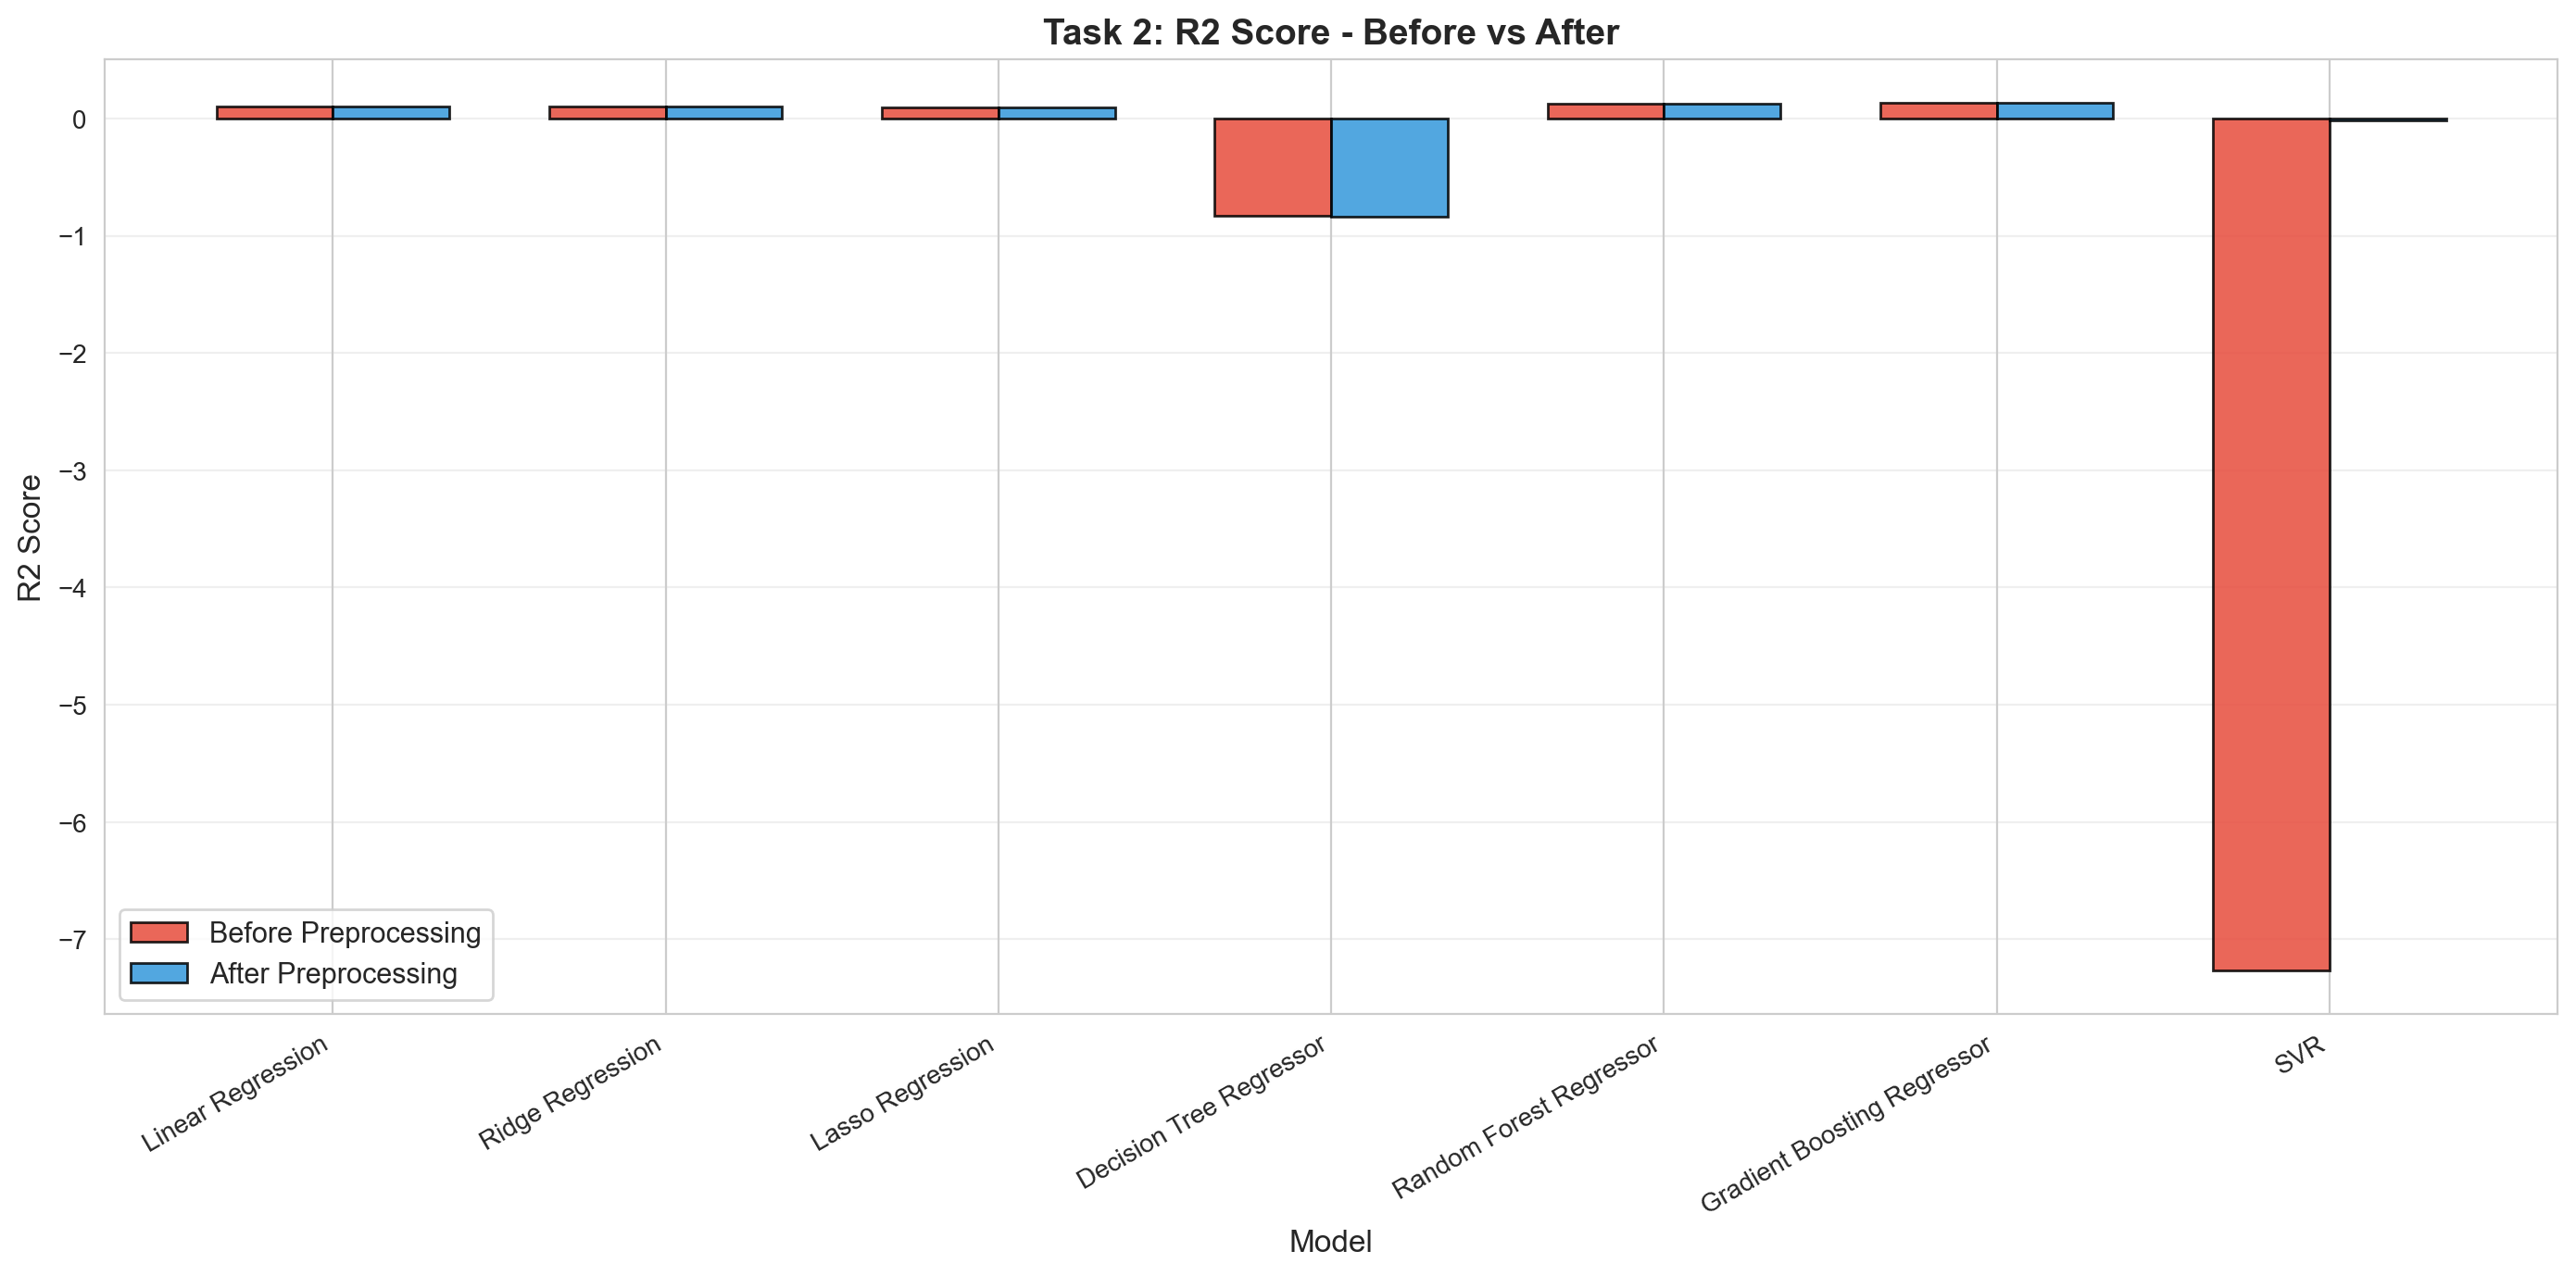
\includegraphics[width=0.7\textwidth]{figures/fig_task2_r2_comparison.png}
    \caption{$R^2$ comparison for Task 2 regression models.}
\end{figure}

\begin{figure}[H]
    \centering
    
\includegraphics[width=0.65\textwidth]{figures/fig_task2_pred_vs_actual.png}
    \caption{Predicted versus actual values for the best Task 2 model.}
\end{figure}

\FloatBarrier

\subsection{Task 3: Discovering Natural Groupings of News Articles}

Task 3 explored whether the dataset contains natural clusters of articles based on the selected
features. K-Means and DBSCAN were applied and evaluated primarily using the silhouette score.

The elbow method was first used to assess candidate values of $k$ for K-Means. The highest
silhouette score was obtained for $k=2$, where K-Means achieved a silhouette score of 0.4067.
Cluster profiling showed one dominant cluster containing most of the articles and one much
smaller subgroup with stronger topic and keyword-related characteristics.

DBSCAN identified 11 clusters and 9741 noise points, but produced a much lower silhouette
score of 0.0359 when noise points were excluded. This indicates that DBSCAN was less effective
for this dataset.

Overall, K-Means performed better than DBSCAN, but the clustering results suggest that the
dataset does not contain strongly separated natural article groups. Instead, article characteristics
appear to vary more continuously across the feature space.

\begin{figure}[H]
    \centering
    
\includegraphics[width=0.62\textwidth]{figures/fig_task3_clustering_elbow.png}
    \caption{Elbow analysis for Task 3 clustering.}
\end{figure}

\begin{figure}[H]
    \centering
    
\includegraphics[width=0.62\textwidth]{figures/fig_task3_kmeans_clusters.png}
    \caption{K-Means clustering result for Task 3.}
\end{figure}

\begin{figure}[H]
    \centering
    
\includegraphics[width=0.62\textwidth]{figures/fig_task3_dbscan_clusters.png}
    \caption{DBSCAN clustering result for Task 3.}
\end{figure}

\FloatBarrier

\subsection{Task 4: Identifying Content Patterns Associated with High Engagement}

Task 4 used association rule mining to identify feature combinations that tend to appear in
high-share articles. Using binary indicators and a binarized target variable, the Apriori algorithm
produced 27 frequent itemsets and 7 rules with lift greater than 1.01.

Among the most meaningful rules, weekend publication, technology channel membership, and
Friday publication showed positive association with high-share outcomes. In particular, the rule
\textit{is\_weekend $\Rightarrow$ shares\_high} achieved confidence 0.7146 and lift 1.3393,
showing a noticeably higher likelihood of popularity for weekend articles.

Although some rules were trivial due to the structure of binary weekday indicators, the
non-trivial rules still provided useful insights into content characteristics associated with stronger
engagement.

\begin{figure}[H]
    \centering
    
\includegraphics[width=0.68\textwidth]{figures/fig_task4_association_rules.png}
    \caption{Association rule mining results for Task 4.}
\end{figure}

\FloatBarrier

\subsection{Task 5: Optimizing Article Formatting and Media Usage for Maximum Reach}

Task 5 focused on a smaller set of structural article features:
\textit{n\_tokens\_title}, \textit{n\_tokens\_content}, \textit{num\_imgs},
\textit{num\_videos}, \textit{num\_hrefs}, and \textit{num\_self\_hrefs}.
The goal was to understand how article formatting and media usage relate to shares.

\begin{table}[H]
\centering
\caption{Task 5 regression results using structural formatting features}
\begin{tabular}{lcccc}
\toprule
Model & RMSE$_{\log}$ & MAE$_{\log}$ & $R^2$ & RMSE$_{\text{orig}}$ \\
\midrule
Ridge Regression & 0.9171 & 0.7011 & 0.0189 & 11080.36 \\
Lasso Regression & 0.9177 & 0.7011 & 0.0176 & 11083.98 \\
Random Forest Regressor & 0.9417 & 0.7261 & -0.0346 & 11042.59 \\
Gradient Boosting Regressor & 0.8981 & 0.6867 & 0.0591 & 11047.83 \\
\bottomrule
\end{tabular}
\end{table}

The relatively low $R^2$ values show that formatting variables alone explain only a limited part
of the variation in shares. However, the coefficient-based and feature-importance analyses still
provided useful directional insights. Links and images showed positive associations with higher
engagement, while title length and self-references showed weaker or negative associations in some
models.

These results suggest that formatting and media usage matter, but they are not sufficient by
themselves to fully explain article popularity.

\begin{figure}[H]
    \centering
    
\includegraphics[width=0.68\textwidth]{figures/fig_task5_feature_importance.png}
    \caption{Feature importance for Task 5 formatting analysis.}
\end{figure}

\FloatBarrier

\subsection{Task 6: Recommending the Optimal Publication Window}

Task 6 investigated whether content, sentiment, and topic-related features could help distinguish
between weekday and weekend publication patterns. This was treated as a binary classification
task.

\subsubsection*{Results Before Preprocessing}

\begin{table}[H]
\centering
\caption{Task 6 publication window results before preprocessing}
\begin{tabular}{lccccc}
\toprule
Model & Accuracy & Precision & Recall & F1 & ROC-AUC \\
\midrule
Logistic Regression & 0.8691 & 0.0000 & 0.0000 & 0.0000 & 0.5514 \\
Random Forest & 0.8716 & 0.7174 & 0.0318 & 0.0609 & 0.6022 \\
Gradient Boosting & 0.8700 & 0.6296 & 0.0164 & 0.0319 & 0.6260 \\
SVM & 0.8691 & 0.0000 & 0.0000 & 0.0000 & 0.5368 \\
\bottomrule
\end{tabular}
\end{table}

\subsubsection*{Results After Preprocessing}

\begin{table}[H]
\centering
\caption{Task 6 publication window results after preprocessing}
\begin{tabular}{lccccc}
\toprule
Model & Accuracy & Precision & Recall & F1 & ROC-AUC \\
\midrule
Logistic Regression & 0.8691 & 0.0000 & 0.0000 & 0.0000 & 0.5545 \\
Random Forest & 0.8720 & 0.7255 & 0.0356 & 0.0680 & 0.6203 \\
Gradient Boosting & 0.8700 & 0.6296 & 0.0164 & 0.0319 & 0.6251 \\
SVM & 0.8702 & 1.0000 & 0.0087 & 0.0172 & 0.5646 \\
\bottomrule
\end{tabular}
\end{table}

Random Forest performed best on this task with an accuracy of 0.8720 after preprocessing.
However, this result should be interpreted carefully because the dataset is highly imbalanced
between weekday and weekend articles. The very low recall values for the weekend class indicate
that the models struggled to identify weekend articles reliably. Therefore, this task is more
appropriately treated as an exploratory investigation than as a strong recommendation model.

\begin{figure}[H]
    \centering
    
\includegraphics[width=0.68\textwidth]{figures/fig_task6_roc.png}
    \caption{ROC curve for Task 6 publication window classification.}
\end{figure}

\begin{figure}[H]
    \centering
    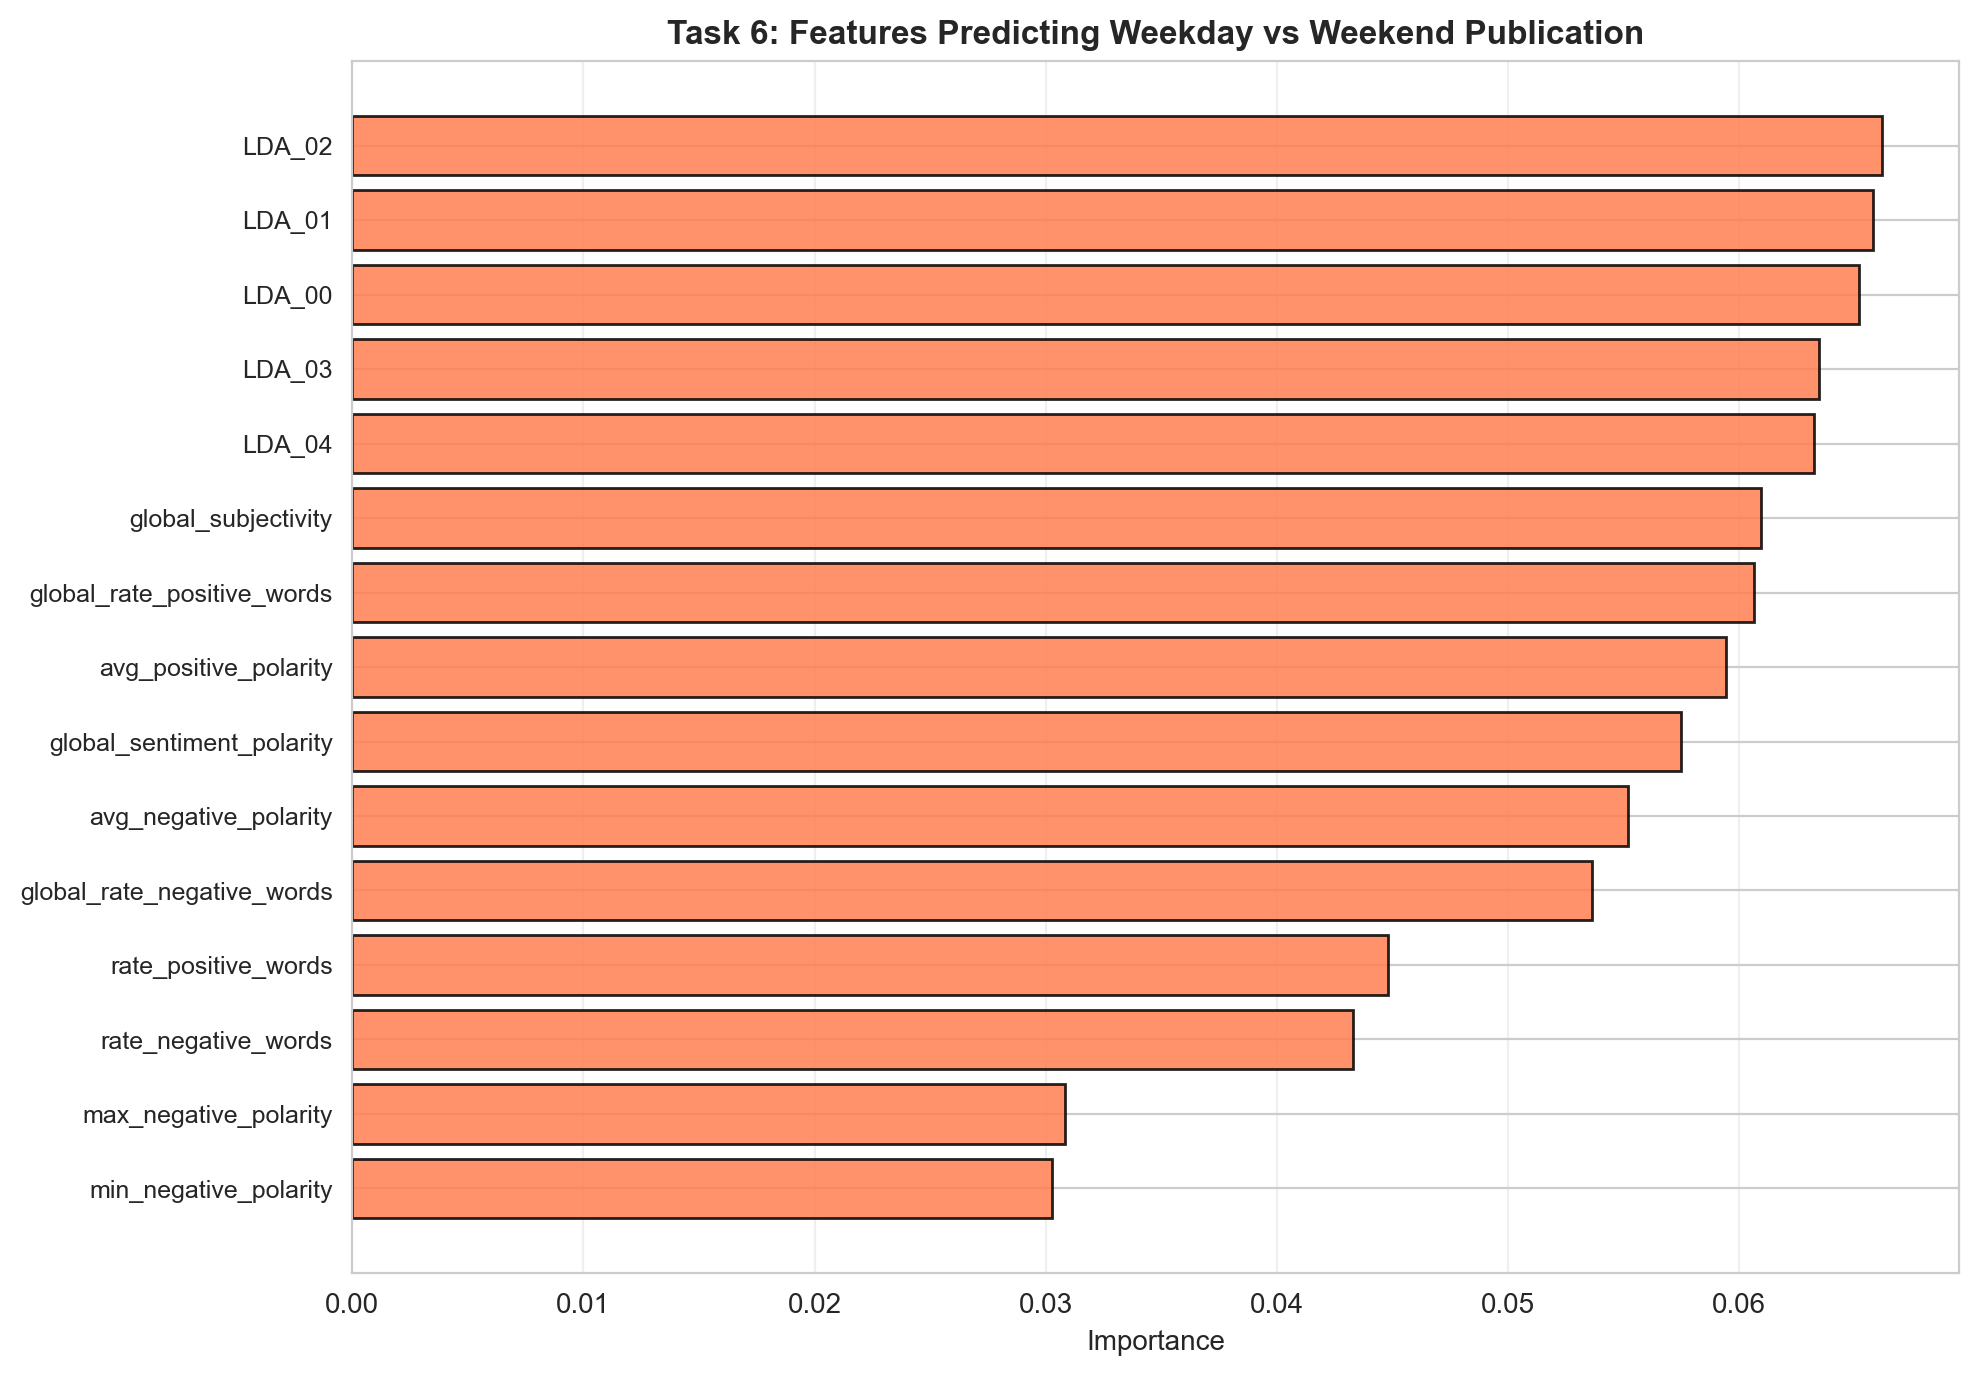
\includegraphics[width=0.68\textwidth]{figures/fig_task6_feature_importance.png}
    \caption{Feature importance for Task 6.}
\end{figure}

\FloatBarrier

\subsection{Scalability Demonstration with Spark}

In addition to the six analytical tasks, a Spark-based scalability demonstration was performed
to show how the workflow can be extended to distributed environments. A Spark Random Forest
classifier was trained using the same popularity threshold as Task 1.

The Spark model achieved an accuracy of 0.6539 and a ROC-AUC of 0.7087, which are very
close to the corresponding scikit-learn Random Forest results. This shows that the analytical
pipeline can be transferred to a distributed framework while maintaining comparable predictive
performance.

The demonstration shows how the same workflow could be scaled to much larger article datasets in future work.